
\documentclass{article}

\usepackage{transparent}
\usepackage{graphicx}
\usepackage{anysize}
\usepackage[spanish]{babel}
\marginsize{1cm}{3cm}{0cm}{0cm}


\usepackage{eso-pic}
\newcommand\BackgroundPic{
\put(0,0){
\parbox[b][\paperheight]{\paperwidth}{%
\vfill
\centering
\color{red}%
\transparent{0.9}%
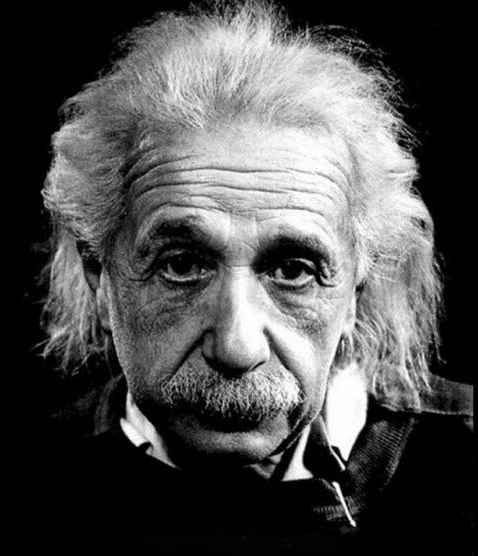
\includegraphics[width=\paperwidth,height=\paperheight,
keepaspectratio]{eisten.png}%
\vfill
}}}


\title{A Small \LaTeX{} Article Template\thanks{To your mother}}
\author{L. González-Santos  \	Instituto de Neurobiología, UNAM  
	}

\date{\today}
% Hint: \title{what ever}, uthor{who care} and \date{when ever} could stand 
% before or after the egin{document} command 
% BUT the \maketitle command MUST come AFTER the egin{document} command! 


\begin{document}

\AddToShipoutPicture{\BackgroundPic}

\maketitle
\begin{enumerate}
\item Como entrar a una terminal de usuario en Windows, MAC o Linux

\item listar el contenido del HOME

\item ¿Cuáles son los tres componentes principales de una computadora?

\item Enumere tres lenguajes de programación y compare sus diferencias. ¿Por qué hay tantos lenguajes de programación?

\item ¿Cómo se pueden iniciar las interfaces de usuario de texto en Windows, Linux y Mac OS?

\item Realice lo siguiente en una interfaz de usuario de texto

a) Mostrar la carpeta de trabajo actual.
b) Ingrese a la carpeta "HOME".
c) Ingrese a la carpeta "Desktop"
d) Cree una nueva carpeta con el nombre Nuevo en la carpeta Escritorio y verifique que aparezca en el escritorio gráfico.

\item Inicie el programa python y luego ciérrelo.
\end{enumerate}



\end{document}
